\section{Proyecto principal}
%
%
Este trabajo trataba de la optimización del gasto energético de una empresa que contaba con hornos de fundición. Para ello, se tuvieron que realizar predicciones del precio de la electricidad mediante modelos estadísticos. Posteriormente, se modelizó el proceso de fundición llevado a cabo en la fábrica y por último se trató de optimizar la selección de los materiales a fundir, dependiendo del espacio disponible en fábrica y el precio de la luz en cada tramo horario, estimado previamente.\\

Por motivos de extensión, y porque es la parte a la que más tiempo he dedicado, la sección asociada a la predicción de precios de la luz será la más extensa y detallada. Respecto del modelado y proceso de optimización se explicará más brevemente, además de que puden incluir información privada del cliente por lo que no se incidirá demasiado.
%
%
\subsection{Predicción de precios de la luz}
%
%
%
%
Para llevar a cabo un modelo predictivo de de los precios de la luz para una empresa hemos de realizar una serie de pasos. En primer lugar, como es evidente, debemos conocer y entender qué es lo que queremos predecir, bajo qué condiciones y qué variables afectan al precio de la luz, tanto naturales, como puede ser la demanda, la generación de ciertos tipos de energía, como aquellas relacionadas con la legislación vigente. Posteriormente debemos decidir cómo se extraeran los datos necesarios. Puesto que estamos hablando de un proyecto real, la empresa espera un proceso automatizado por lo que se debe tener en cuenta una extracción periódica de datos.\\

Una vez planteado el contexto en el que vamos a movernos, debemos decidir qué modelos probar, conociendo sus ventajas y desventajas. Mi elección, basada en búsquedas de desarrollos similares, fue optar por tres modelos:
\begin{description}
    \item[SARIMAX] Modelo estadístico clásico
    \item[XGBoost] Modelo de \textit{machine learning}
    \item[TFT] Modelo de \textit{deep learning}
\end{description}

Por último, por requisitos del proyecto, la predicción se realizaba a un mes vista, lo cual como es lógico, no es óptimo. Sin embargo, esto era algo fijo por lo que los resultados esperados son mejorables, recortando el horizonte de predicción y reentrenado los modelos con mayor asiduidad.
%
%
%
\subsubsection{Estudio y comprensión del mercado}
%
%
%
Dado que la empresa es una electrointensiva no se rige por el régimen general del pequeño consumidor (PVPC). Para la toma de datos de la variable objetivo, el precio de la luz, se consultó el precio del mercado SPOT diario, que es el que regula la venta de luz al por mayor.\\

Para calcular exactamente, dentro de lo que podemos entender como \textit{exacto} en un modelo de predicción, el precio de la luz debemos tener en cuenta tanto el precio de venta como los peajes. Estos últimos son valor añadido a la factura de la luz que depende del tipo de empresa y de la hora de consumo. De cualquier forma, en lo que a nuestro modelo se refiere, únicamente nos interesa el preio del mercado SPOT diario, que viene dado de manera horaria.
%
%
%
\subsubsection{Obtención y preparación de los datos}
%
%
%
Los datos se obtuvieron a través de la API pública proporcionada por ESIOS (Sistema de Información del Operador del Sistema Eléctrico), que permite acceder a los precios horarios históricos, así como a otros indicadores del sistema eléctrico. De manera adicional al precio de la luz, y como se ha comentado previamente, se tomaron variables explicativas, es decir, que se cree que tienen relación y afectan al precio de la que queremos. En este caso, se tomó: La demanda real de consumo, la generación de energía eólica y solar.\\

En lo relativo a la preparación de los datos, salvando las diferencias en función de la implementación del modelo, el procedimiento fue similar: Una vez descargados los datos se formatean de manera que tengamos aquellos valores que queremos, es decir, el precio, demanda, etc. y la fecha en la que se dio. Además, de cara a refinar nuestro modelo, se introdujeron variables temporales como el día de la semana, día del mes o mes del año. Un estudio mucho más exaustivo puede hacerse incluyendo más variables o con más combinaciones. En \cite{TFG_prediccion} puede verse como incluyen el precio del gas o la emisión de CO$_2$ entre otro, llevándoles a mejores resultados, aunque con mayor trabajo.
%
%
%
\subsubsection{Análisis exploratorio}
%
%
%

%
%
%
\subsubsection{SARIMAX}
%
%
%
Este es un modelo modelo autorregresivo que incorpora la relación de la variable endógena (el precio de la luz) con sus \textit{lags} (rezazgos) y variables exógenas que pueden influir sobre él. La ventaja de este modelo es que es relativamente sencillo de implementar y de entender, por lo que permite una gran manejabilidad en cuanto a los parámetros a introducir y los resultados obtenidos.\\

El modelo SARIMAX se basa en varias suposiciones clave. La más importante es que la serie de datos sea \textit{estacionaria}. Esto significa que sus propiedades estadísticas, como la media y la varianza, deben ser constantes a lo largo del tiempo. Además, se asume que los residuos del modelo son ruido blanco, es decir, que son independientes e idénticamente distribuidos, con media cero y varianza constante. También se considera que no hay autocorrelación en los residuos.\\

El modelo SARIMAX viene caracterizado por los parámetros $(p,d,q)x(P,D,Q,s)$ donde:
\begin{itemize}
    \item[$p$]: Orden del componente autorregresivo (AR) no estacional. Indica el número de rezagos de la variable endógena que se incluyen en el modelo.
    \item[$d$]: Orden de diferenciación no estacional. Representa la cantidad de veces que se deben diferenciar los datos para hacer la serie estacionaria.
    \item[$q$]: Orden del componente de media móvil (MA) no estacional. Indica el número de rezagos del error del pronóstico que se incluyen en el modelo.
    \item[$P$]: Orden del componente autorregresivo (AR) estacional.
    \item[$D$]: Orden de diferenciación estacional.
    \item[$Q$]: Orden del componente de media móvil (MA) estacional.
    \item[$s$]: Período de estacionalidad, en este caso vemos que $s=24$ de manera natural al tratarse de precios horarios.
\end{itemize}

Para determinar los órdenes de los parámetros del modelo, se analizan las funciones de autocorrelación (ACF) y autocorrelación parcial (PACF). La ACF mide la correlación de la serie consigo misma en diferentes rezagos, mientras que la PACF mide esta misma correlación eliminando la influencia de los rezagos intermedios.\\

En las siguientes imágenes podemos ver los gráficos de ACF y PACF para la serie de precios de la luz, lo que nos permite identificar los patrones de estacionalidad y los órdenes de los modelos.

\begin{figure}[H]
    \centering
    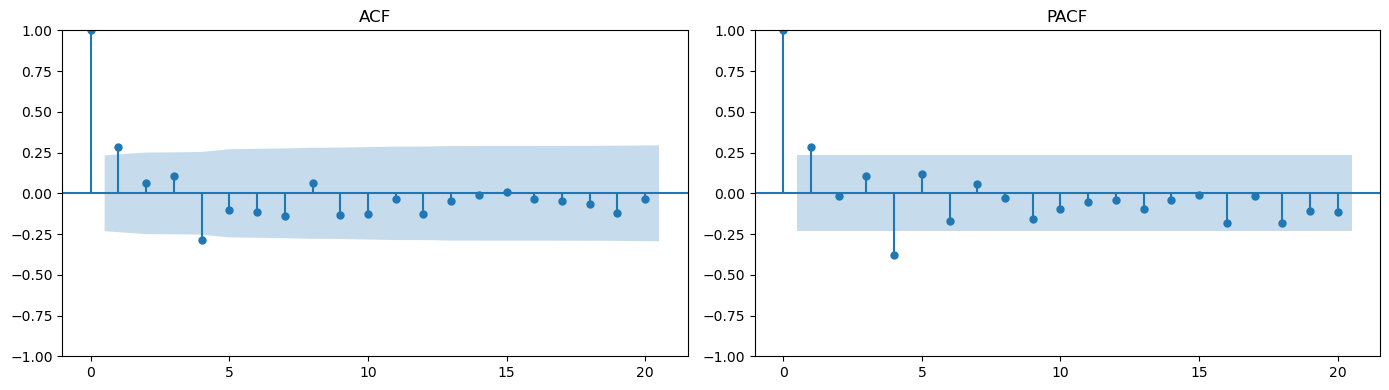
\includegraphics[width=0.7\linewidth]{figuras/ACF_PACF.png}
    \caption{ACF y PACF de la serie de precios de la luz sin diferenciar. Se observa una clara estacionalidad y una autocorrelación que decae lentamente, lo que sugiere la necesidad de diferenciación.}
    \label{fig:ACF_sin_diferenciar}
\end{figure}
\begin{figure}[H]
    \centering
    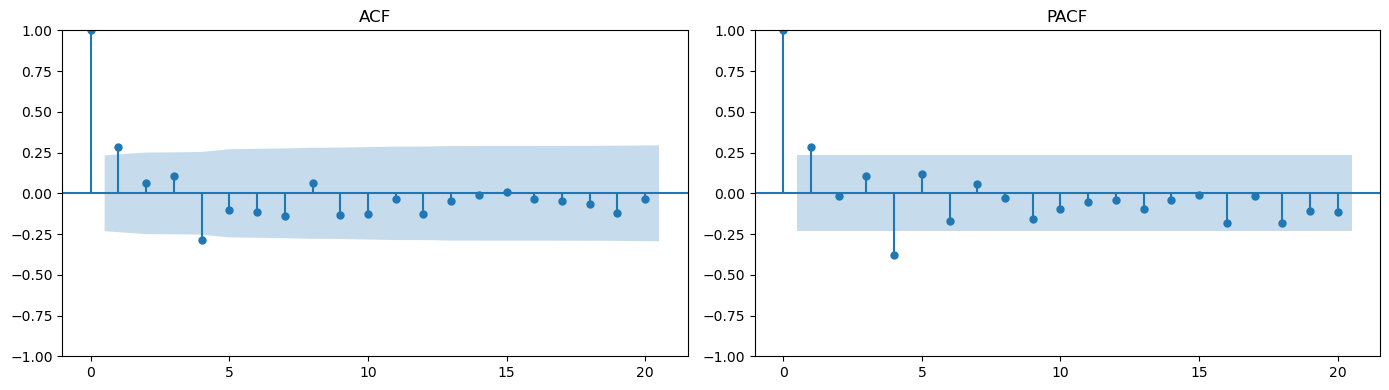
\includegraphics[width=0.7\linewidth]{figuras/ACF_PACF.png}
    \caption{ACF y PACF de la serie de precios con diferenciación estacional. Aunque la estacionalidad ha sido eliminada, la autocorrelación no estacional aún persiste.}
    \label{diferenciado}
\end{figure}
\begin{figure}[H]
    \centering
    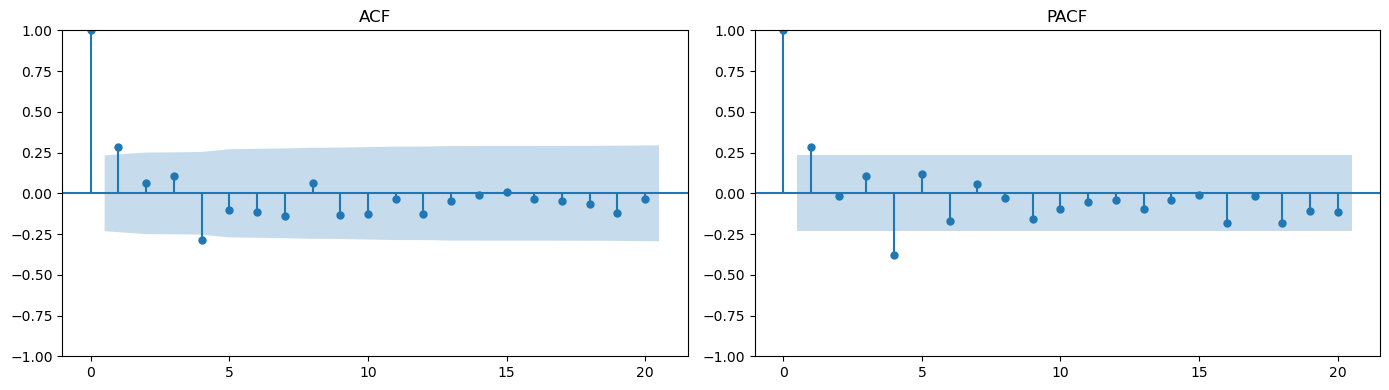
\includegraphics[width=0.7\linewidth]{figuras/ACF_PACF.png}
    \caption{ACF y PACF de la serie con diferenciación doble. Ahora la serie es estacionaria y los rezagos significativos nos indican los posibles órdenes $p, q, P, Q$.}
    \label{dobledifereniado}
\end{figure}

Basado en el análisis de las funciones de autocorrelación, se han preseleccionado los siguientes tres modelos con sus respectivos parámetros:

\begin{itemize}
    \item \textbf{Modelo 1: SARIMAX(1,1,1)x(1,1,1,24)}:
    Se elige este modelo porque los picos en los gráficos de ACF y PACF de la serie doblemente diferenciada son significativos en el primer rezago no estacional y estacional. Esto sugiere un orden de 1 para los componentes AR, MA, y sus contrapartes estacionales.

    \item \textbf{Modelo 2: SARIMAX(0,1,1)x(0,1,1,24)}:
    Este modelo se considera debido a que, en el gráfico PACF, los picos son más pronunciados en los primeros rezagos, lo que podría indicar la preponderancia de los términos de media móvil.

    \item \textbf{Modelo 3: SARIMAX(2,1,0)x(2,1,0,24)}:
    Se opta por este modelo como alternativa, ya que los gráficos de ACF y PACF también muestran una posible influencia de los segundos rezagos, tanto estacionales como no estacionales.
\end{itemize}

Estos tres modelos serán evaluados y comparados utilizando métricas como el MAE y el RMSE para determinar cuál de ellos ofrece un mejor ajuste a los datos.
%
%
%
\subsubsection{XGBoost}
%
%
%
Este modelo, basado en árboles de decisión, también relativamente sencillo de implementar aunque, como es habitual en este tipo de modelos, menor interpretabilidad de lo que ocurre dentro del algoritmo. Su robustez viene por la capacidad de aprender patrones complejos pero mejorado mediante técnicas de aproximación en las funciones de pérdida y regularización. Esta segunda suele ser la primera que se mira cuando se trata de modelos predictivos puesto que habla de la precisión del mismo, sin embargo, XGBoost permite la regularización de manera que evitemos el \textit{overfitting} (sobreajuste), es decir, que durante la etapa de entrenamiento el modelo adopte patrones demasiado complejos, propios del conjunto introducido de manera que pierda generalidad y por ello no sea capaz de realizar buenas predicciones.
%
%
%
\subsubsection{TFT}
%
%
%
Este modelo es uno de los más avanzados, estado del arte en diversas áreas. Su funcionamiento es más complejo aunque puede entenderse la estructura (ver pre-print original \cite{TFT}). Por dar una breve explicación
%
%
%

\subsubsection{Resultados}
%
%
%

%
\subsection{Modelo físico}
%
%
\subsubsection{Situación simplificada: Primera aproximación} \label{PrimeraAproximacion}
%
%
%
Dado un metal conocido (X) de temperatura de fusión $T_f$, calor específico en los estados sólido y líquido, $c_{\text{sol}}$ y $c_{\text{liq}}$ respectivamente, entonces a la hora de conocer cuánta energía será necesaria tendremos que tener en cuenta:
\begin{itemize}
    \item[I] El metal X a una temperatura inicial $T_0$ debe ser calentado hasta la temperatura de fusión $T_f$, esto dependerá del \textit{calor específico} del material en el estado \textit{sólido}, que viene a ser el \textit{coste} energético para aumentar la temperatura del mismo.
    \item[II] Una vez alcanzado dicho objetivo el material cambia de estado de la materia requiriendo una nueva cantidad de calor dependiente del \textit{calor latente} del material, denominado como $L_{\text{s-l}}$.
    \item[III] Finalmente supondremos que seguiremos elevando la temperatura por lo que, de manera análoga al paso I, tendremos que tener en cuenta esta energía. Llamaremos a este límite $T_c$
\end{itemize}
Para realizar dichos cálculos, haremos uso de las fórmulas de calor para calor específico y transiciones de fase.
\begin{align}
    Q_{\text{pf}} &= m \cdot c_{\text{sol}} \cdot (T_f-T_0).\\
    Q_{\text{f}} &= m \cdot L.\\
    Q_{\text{e}} &= m \cdot c_{\text{liq}} \cdot (T_c-T_f).
\end{align}
De este modo, $Q = Q_{\text{pf}} + Q_{\text{f}} + Q_{\text{e}}$. Finalmente, deberíamos tener en cuenta que los hornos no son ideales y tenemos una cierta pérdida de energía. Este hecho, cuantificado por el rendimiento $\eta \in [0,1]$, provoca un aumento en el calor total necesario: $Q^{\text{tot}} = Q/\eta$.

\subsubsection{Situación general} \label{SituacionGeneral}
%
%
%
Nos situamos ahora ante el problema general, en el que partimos de temperaturas iniciales cercanas a la ambiente ($T_0 \simeq 25 \C$) mientras que llegamos por lo menos a $T = 1450 \C$. En este caso tendremos que aplicar la formulación general:
\begin{equation}
    Q = m \cdot \int_{T_a}^{T_b} c(T)dT,
    \label{calor}
\end{equation}
donde $m$ es la masa del compuesto X y $c(T)$ es la función del calor específico con la temperatura. Para poder operar con esta expresión sería necesario consultar datos tabulados sobre el material y una vez obtenidos los datos de $c$ para distintas temperaturas interpolamos obtener una función con la que calcular, de manera aproximada, el calor en la \Cref{calor}.
De este modo llegaríamos a una situación similar a la descrita en la \Cref{PrimeraAproximacion}, obteniendo $Q^{\text{tot}}$. En ambos casos, como se va a tener desarrollo polinómico de $c(T)$, podemos calcular
\begin{align}
    Q & = m \cdot \int_{T_a}^{T_b} c(T)dT = m \cdot \int_{T_a}^{T_b} \Big[a_0+ a_1 T + \dots + a_nT^n \Big]dT = \\
    & = m \cdot \Big[a_0T+ \frac{a_1}{2} T^2 + \dots + \frac{a_n}{n+1} T^{n+1}\Big] \bigg|_{T_a}^{T_b} = m \cdot p(T_a, T_b),
\end{align}
donde sustituyendo obtenemos el valor deseado. Para el primer caso, tenemos que $T_a$ coincide con la temperatura \textit{ambiente} de la pieza mientras que $T_b$ con la de fusión del material X. Por otro lado, para la etapa final, la temperatura de fusión coincide con la inicial y la final, supondremos que es $1450 \C$ para todas las piezas.
\subsubsection{Traducción matemática}
La situación anterior debe ser convenientemente planteada como restricciones, de cara a la resolución del problema de optimización con el que nos encontramos. Aunando lo descrito en la \Cref{SituacionGeneral} podemos escribir que el calor $Q$ necesario para la pieza X es:
\begin{equation}
    Q = Q_{\text{pf}} + Q_{\text{f}} + Q_{\text{e}} + Q' = m \cdot \Big( p_I + L + p_{III} \Big) + Q',
\end{equation}
Donde el término $Q'$ es la energía debida a un requerimiento del fabricante, tanto de precalentamiento como de pos-fundición.\\

Finalmente, debería considerarse el rendimiento $\eta$ de los hornos. Supondremos, salvo que se indique lo contrario, que ambos hornos presentan el mismo rendimiento. Adicionalmente, dado que este valor es una constante, tenemos que $\min{\eta f(x)} = \eta \min{f(x)}$ por lo que prescindiremos de este valor puesto que no influye en la función objetivo y únicamente debería ser considerado en última instancia, a la hora de predecir el gasto estimado. Ya por último, se ha obtenido el calor $Q$ con unidad (J) \textit{julios}, mientras que habitualmente el coste eléctrico se da en \euro/kWh por lo que deberemos realizar la debida conversión. Esta, al igual que pasa con el rendimiento, influye en el valor numérico final pero no en el problema a optimizar.
%
%
\subsection{Optimización de la superficie de enfriamiento}
%
%
El presente problema aborda la distribución de las piezas metálicas recién fundidas sobre la superficie de enfriamiento disponible en la nave. Cláramente, el objetivo es maximizar el número total de piezas que pueden colocarse simultáneamente. Esta superficie cuenta además con restricciones físicas relacionadas con la seguridad y operatividad del proceso, como márgenes laterales y pasillos interiores obligatorios de al menos 1.5 metros de ancho.\\

Cada pieza fundida es clasificado según su diametro y para su manipulaciónha sido previamente colocada en una caja cuya dimensión se determina en función del tipo correspondiente. Estas cajas se disponen en planta sobre la superficie, sin posibilidad de apilarse. Una vez colocadas, las cajas no pueden solaparse ni invadir los pasillos o márgenes de seguridad. Es decir, deben respetarse las distancias mínimas entre ellas y con respecto a los bordes del área de enfriamiento. Esto impone restricciones geométricas estrictas sobre su posicionamiento.\\

El objetivo final es obtener una disposición óptima que maximice la cantidad total de piezas colocadas, permitiendo una planificación eficiente del enfriado. Dado el carácter discreto y combinatorio del problema, este puede abordarse mediante algoritmos de optimización específicos como métodos de empaquetado 2D, algoritmos genéticos o formulaciones de programación entera si se requiere una solución exacta.\\
%
%
